\IfFileExists{generated/tab_prev_court_full.tex}{\input{generated/tab_prev_court_full}}{}


\subsection{What the population looks like} Figure \ref{fig:funnel} gives the eligibility funnel. Of \NScanned{} opinion records in the bulk table,
\NFedApp{} belong to the fourteen courts and carry extractable text, and
\NEligible{} survive the eligibility criteria. The largest single reduction is
the thousand-character minimum, which removes short orders and judgment entries;
Supreme Court records account for a disproportionate share of these, because
orders-list entries are stored as opinions. Deduplication removes a further
tranche of records that are the same opinion ingested from more than one source.

\subsection{How often courts say they are not deciding} \NWithTrigger{} eligible
opinions, or \Prevalence{}, contain at least one of the thirteen expressions,
with \NOccurrences{} occurrences in total across \NWordsBn{} billion words.
Figure \ref{fig:trigger} breaks this down by expression and Table
\ref{tab:prevcourt} by court. The rate is not uniform, running from
\CourtLoRate{} in the \CourtLo{} to \CourtHiRate{} in the \CourtHi{}.


\begin{figure}[t]
\centering
\IfFileExists{generated/fig_time.pdf}{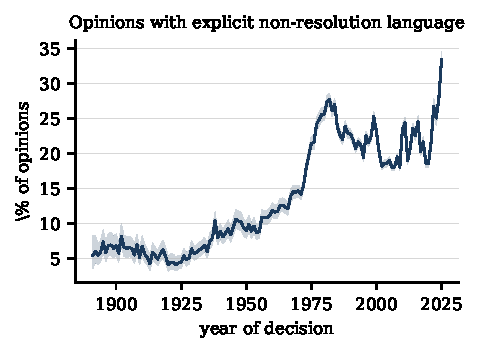
\includegraphics[width=0.88\columnwidth]{generated/fig_time.pdf}}{\fbox{\parbox{0.9\columnwidth}{\centering\vspace{2em}[figure pending]\vspace{2em}}}}
\caption{Share of eligible federal appellate opinions containing at least one
frozen dictionary expression, by year of decision, with Wilson intervals. Years
with fewer than 150 eligible opinions are omitted.}
\label{fig:time}
\end{figure}

 Figure \ref{fig:time} and Table \ref{tab:prevperiod} give
the temporal picture. Both the opinion-level rate and the rate per hundred
thousand words are reported, because opinion length is not constant across eras
and an opinion-level rate alone confounds the two. The corpus itself changes over
this span, in coverage, in digitization source, and in the share of unpublished
dispositions, so the series should be read as a property of the available record
rather than as a clean measurement of judicial behaviour over two centuries.

Opinion type and precedential status were named as secondary analyses before the corpus was built; Appendix \ref{app:prev} reports both.


\begin{figure}[t]
\centering
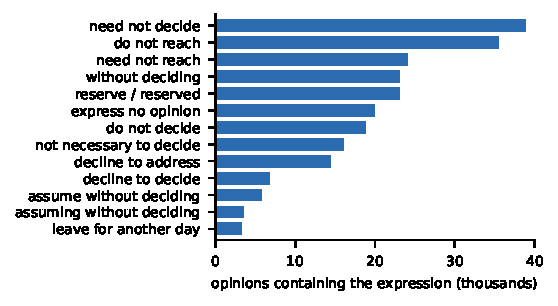
\includegraphics[width=\columnwidth]{generated/fig_trigger.pdf}
\caption{Opinions containing each of the thirteen frozen expressions. T08 and T09 are subsets of T07 by construction.}
\label{fig:trigger}
\end{figure}

\section{Building the Benchmark}
\label{sec:bench}

If the negative class is
passages without a trigger, the task reduces to phrase recognition and
any result is about the dictionary rather than about disposition. Three moves
address this.

\subsection{Matched controls}
For each trigger-bearing opinion we draw a control opinion containing no
dictionary expression anywhere, matched on court, period, opinion type, and
length decile, and locate an issue inside it. Two locators are used: a holding
cue (\textsc{ctrl\_hold}) and a neutral marker naming an issue without
indicating how it came out (\textsc{ctrl\_rand}), so the benchmark stands
independent of the assumption that decided issues are the ones near ``we
hold.''

\subsection{Adversarial strata}
Two structural flags identify passages where the dictionary is likely to
mislead. H1 marks a trigger whose subject is plausibly another institution or
that sits inside a quotation. H2 marks a trigger followed later in the same
opinion by a holding sentence about the same proposition, the shape of a court
that says it need not decide and then decides. Neither flag assigns a label;
both are sampling strata, and annotation settles what the passage does.

\subsection{Neutral issue statements}
Each item carries a statement of the proposition at stake, constructed so it
cannot leak the answer: any dictionary expression or holding cue is cut before
the statement is kept. Appendix \ref{app:issue} gives the procedure and the
\ExtractYield{} yield.

\IfFileExists{generated/tab_stratum_full.tex}{\begin{table}[t]
\centering\small
\begin{tabular}{lrrrr}
\toprule
stratum & dec. & unres. & unclear & \% unres. \\
\midrule
CTRL\_HOLD & 72 & 0 & 1 & 0.0 \\
CTRL\_RAND & 14 & 0 & 16 & 0.0 \\
H1 & 10 & 57 & 31 & 85.1 \\
H2 & 6 & 59 & 0 & 90.8 \\
PLAIN & 5 & 83 & 10 & 94.3 \\
\bottomrule
\end{tabular}
\caption{Annotated labels by sampling stratum. The last column excludes \textsc{unclear}.}
\label{tab:stratum}
\end{table}
}{}


\subsection{Sampling and splits} \NDrawn{} items were drawn with at most one per
opinion, so context windows never overlap and splits are disjoint at the opinion
level. Allocation across strata follows the pilot (Appendix \ref{app:pilot}).
Splits are nested and fixed in order: every item from \HeldOutCourts{} forms the
court-held-out condition, then every remaining item filed in \TemporalCut{} or
later forms the temporal condition, and what is left is split at random into test
and development. Only the development portion was used to fit anything.

\subsection{Annotation} \NAnnotated{} items were annotated under the frozen
guideline, \NUnclear{} of them \textsc{unclear}, leaving \NBench{} with a
usable binary label. Items were presented in a fixed random order ignoring
stratum, split, court, and period, so the annotated set is a random subsample of
what was drawn. Table \ref{tab:stratum} gives labels by stratum.


\section{Can Models Tell?}
\label{sec:models}

\IfFileExists{generated/tab_models_full.tex}{\input{generated/tab_models_full}}{}


\subsection{Systems} Five are compared at four context widths: the frozen
dictionary as a floor; TF-IDF with logistic regression and two fine-tuned
encoders, supervised on the \NDev{}-item development split; a zero-shot open
model, \LLMName{}, scored by the likelihood of the two label continuations so it
never generates; and a classifier seeing only the issue statement, as a leakage
control. One system is deliberately absent: a frontier model would be the natural
comparison, but the only one available here also produced the labels, and a
system evaluated against its own annotations measures nothing.

\subsection{The pooled lexical score is an artefact of our sampling} The frozen
dictionary reaches macro-$F_1$ of \LexF{} on the random test set, which is not a
difficulty measure. Every window is centred on the anchor, so a trigger-bearing
item contains its trigger in every window and a control item contains none. The
rule reduces to ``is this item from the trigger family'': its score is fixed by
the stratum quotas and cannot vary with context width.

\subsection{Supervised systems beat the dictionary where it was built to fail}
On H1, built so the expression is present but is not this court announcing its
own non-resolution, the rule reaches \LexHOne{} while the sparse model reaches
0.947; it also edges the rule on \textsc{plain} (0.962 against 0.942). The
dictionary's pooled advantage comes entirely from the control strata, where it is
correct by construction. The encoders show the pattern more strongly: the best
reaches \BestF{} on the random test set, and on the court-held-out condition
legal-bert reaches 0.975 against the rule's 0.917.

It appeared as the development split
grew, so we measured it directly. Figure \ref{fig:lc} resamples training subsets
of increasing size and evaluates each on the held-out H1 items. Accuracy rises
monotonically, the spread across resamples narrows to nothing, and the share of
subsets beating the dictionary goes from none at 45 items to all of them at
\NDev{}, crossing over near \LCCross{}. That is the shape of a learning curve
rather than of noise, and it says the benchmark is nowhere near saturated.

\begin{figure}[t]
\centering
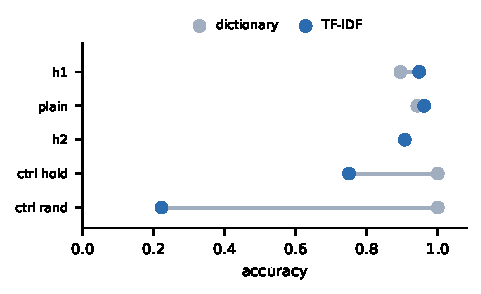
\includegraphics[width=0.88\columnwidth]{generated/fig_strata.pdf}
\caption{Accuracy by sampling stratum at the anchor sentence. The dictionary is at ceiling on the controls by construction; the informative comparison is H1.}
\label{fig:strata}
\end{figure}

\subsection{Context helps up to a point and then hurts} For a window $w$ we
estimate, against the anchor sentence $w_0$,
\begin{equation}
\Delta(w)=F_1\!\left(y,\hat{y}_w\right)-F_1\!\left(y,\hat{y}_{w_0}\right),
\end{equation}
resampling the same items for both conditions, so the comparison is paired and
isolates the window. Table \ref{tab:context} reports it. Widening to $\pm256$
characters costs nothing measurable on the random test set ($-0.014$, 95\% CI
$[-0.110, 0.076]$). Widening further is costly and the effect is clear:
$\pm1024$ costs $-0.245$ and $\pm4096$ costs \CtxWorstDelta{} (95\% CI
$[-0.421, -0.167]$). The zero-shot model traces the same curve, from
\LLMSentF{} at the sentence to \LLMWideF{} at its widest window.

The reading we prefer is that the disposition of one proposition is marked
locally, and that a window wide enough to hold a second issue introduces its
disposition as noise. That is a statement about fixed-window models rather than
about context in principle. A system that locates the later holding sentence rule
L1-3 turns on, rather than consuming everything around it, is left to future
work.


\begin{figure}[t]
\centering
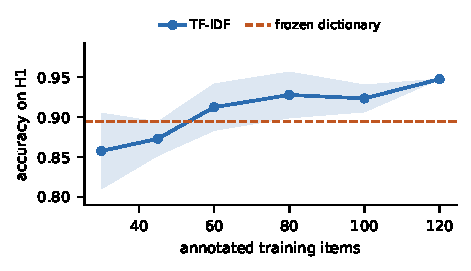
\includegraphics[width=0.82\columnwidth]{generated/fig_lc.pdf}
\caption{Learning curve on the adversarial stratum. Each point resamples twelve training subsets; bars are one standard deviation.}
\label{fig:lc}
\end{figure}

\subsection{Three checks} The issue-only classifier reaches \IssueOnlyF{}
macro-$F_1$ against a majority baseline of 0.392, intervals barely overlapping.
Every dictionary expression and holding cue is stripped from a statement before
it is kept, so this is not lexical leakage but subject matter: which questions
courts decline to reach correlates with what they are about. Part of what looks
like reasoning is available from the topic alone.

Re-annotating \NHumanAbl{} items with only the anchor sentence, the label matches
the full-context label \HumanAgree{} of the time, and every flip falls in H1 and
\textsc{ctrl\_hold}. What changes most is the willingness to answer, abstention
rising from \HumanUnclearFull{} to \HumanUnclearSent{}. For a person as for a
model, context buys confidence more than accuracy.

Courts also label each other. A parenthetical reading ``(declining to decide
whether $X$)'' asserts that the cited case did not resolve $X$, and we harvest
\NCharTight{} such characterizations. They serve as a resource rather than as
validation, since if a later court says \emph{Smith} held $X$ and we say
\emph{Smith} left $X$ open, either our label is wrong or the later court has
overstated \emph{Smith}, and the disagreement is consistent with both. Appendix \ref{app:errors} works through
the cases that separate the systems, selected by a fixed rule rather than by
hand.

\section{What Happens Next to an Unresolved Issue}
\label{sec:long}

Annotating citation chains one at a time does not scale. Of citing passages that
survive a content-word filter, \OffIssueRate{} are still about something other
than the issue, so a usable observation costs roughly ten annotations. Instead we
measure the phenomenon the way \S\ref{sec:prev} measures prevalence, with frozen
dictionaries applied to the whole corpus.

\subsection{Matching propositions, not positions} Asking whether a
non-resolution expression sits near the characterized passage is cheap but wrong:
of \NProxyCheck{} flagged cases only \NProxyGood{} were genuine, the expression
usually governing a neighbouring question (Appendix \ref{app:layer2}). Comparing propositions works. Writing
$C(x)$ for the content words of a text, we match the origin's issue statement $q$
against the later court's characterization $c$ when
\begin{equation}
J(q,c)=\frac{|C(q)\cap C(c)|}{|C(q)\cup C(c)|}\;\geq\;\tau,
\qquad \tau=0.34,
\end{equation}
so both sides of the comparison are propositions rather than positions in a
document. Of \NCharTight{} characterizations only
\NIMMatched{} clear the threshold, few enough to hand-verify each:
\NIMGenuine{} are genuine, \NIMPrec{} precision against \ProxyPrec{}, over
\NIMDistinct{} propositions.

\begin{figure}[t]
\centering
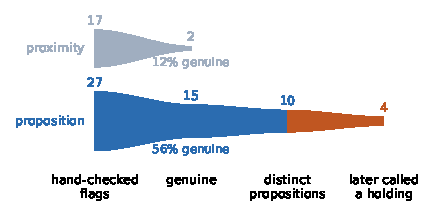
\includegraphics[width=0.74\columnwidth]{generated/fig_escal.pdf}
\caption{Attrition under the two matching strategies. Ribbon thickness is the
count at each stage, so the first taper is the verified precision. The orange
tail is the case series.}
\label{fig:escal}
\end{figure}

\subsection{What the verified cases show} Among those \NIMDistinct{}
propositions, each one a question the originating court demonstrably declined to
decide, \NIMEsc{} are described by a later court as something that court held.
The majority are reported accurately, with the later court repeating the
reservation, as when one opinion notes that \emph{Davis} reserved the question
whether a request for counsel can be rendered ambiguous by preceding events.

Writing $S(o_1,q)\in\{L_0,\dots,L_3\}$ for the status a later opinion $o_1$
ascribes to proposition $q$ and $S_0(q)$ for what the origin did, the quantity of
interest is
\begin{equation}
\Pr\!\left[S(o_1,q)=L_3 \mid S_0(q)=\textsc{unresolved}\right],
\end{equation}
the chance that a question a court declined to decide is later called its
holding. This is a case series and not a rate. Ten propositions cannot support an
interval, and the threshold selects for verbatim quotation and so for the cases
most likely to be characterized accurately, a bias against the phenomenon. It
establishes that escalation occurs and that issue matching, not data, is the
constraint. Appendix \ref{app:layer2} elaborates.

